\section{How does Intel SGX work}

\begin{frame}
    \frametitle{Overview}
    \begin{itemize}[<+->]
        \item Application is split into a secure part and a non-secure part
        \begin{itemize}
            \item Trusted functions processing secrets (e.g. passwords, encryption keys)
            \item Untrusted functions for non-critical computations / procedures
        \end{itemize}
        \item Trusted functions are handled by an ``enclave``
        \item Enclave is launched by the application
        \item Enclave code is called by the application through enclave entry point
    \end{itemize}
\end{frame}

\begin{frame}
    \frametitle{Overview}
    \begin{itemize}[<+->]
        \item Enclaves can be seen as shared objects (.so on Unix, .dll on Windows) which provide trusted functions
        \item Trusted functions should only handle security critical procedures (e.g. password reads)
        \item Enclave memory can only be read by trusted functions
    \end{itemize}
    \centering
    \visible<4>{\incfig[0.4\textwidth]{Enclave}}
\end{frame}

%Quellen unten anpassen
\incfuck[0.8\textwidth]{AppOverview}{1}{{}}{Overview}
\incfuck[0.8\textwidth]{AppOverview}{2}{{}}{Overview}
\incfuck[0.8\textwidth]{AppOverview}{3}{{}}{Overview}
\incfuck[0.8\textwidth]{AppOverview}{4}{{}}{Overview}
\incfuck[0.8\textwidth]{AppOverview}{5}{{}}{Overview}
\incfuck[0.8\textwidth]{AppOverview}{6}{{}}{Overview}
\incfuck[0.8\textwidth]{AppOverview}{7}{{}}{Overview}
\incfuck[0.8\textwidth]{AppOverview}{8}{{}}{Overview}


\begin{frame}
    \frametitle{Implementation: Enclave Page Cache (EPC)}
    \begin{itemize}[<+->]
        \item Code and data of the enclave is stored in a special memory area, called EPC
    \end{itemize}
    

\end{frame}

\begin{frame}
    \frametitle{Implementation}
    \begin{itemize}
        \visible<1->{\item Intel SGX defines 18 new instructions to handle enclaves in hardware}
        \visible<2->{\item Intructions to load enclaves are called through systemcalls, e.g ECREATE}
        \visible<3->{\item Instructions to communicate with the enclave can be called by user, e.g. EENTRY, EEXIT}
        \visible<4->{\item CPU has an extra enclave Mode to call some of these instructions}
        \visible<5>{\item Enclave mode needs a context switch and is for the whole enclave handling and enclave code execution}
    \end{itemize}
\end{frame}

\begin{frame}
    \frametitle{Enclave Page Cache (EPC)}
    \begin{itemize}
        \visible<1->{\item Code and data of the enclave is stored in a special memory area, called EPC}
        \visible<2->{\item This area is encrypted by using the Memory Encryption Engine (MEE)}
        \visible<3->{\item MEE is an extra new and dedicated circuit for Intel SGX}
        \visible<4->{\item Only enclave can read from its own EPC}
        \visible<5->{\item EPC page content is only decrypted inside the CPU}
        \visible<6->{\item Keys for de-/encrypting are generated at boot-time and are stored inside the CPU}
        \visible<7>{\item Enclaves can access their application memory, but not the other way arround}
    \end{itemize}
\end{frame}

\begin{frame}
    \frametitle{Page Check}
    \begin{itemize}
        \visible<1->{\item Page check is extended to prevent external access to EPC}
        \visible<2->{\item The Enclave Page Cache Metadata (EPCM) is stored inside the EPC}
        \visible<3->{\begin{itemize}
            \item EPCM is a map from enclave to pages in the EPC
        \end{itemize}}
    \end{itemize}
\end{frame}

\begin{frame}
    \frametitle{Page Check}
    \begin{figure}
        \centering
        \incfig[0.75\textwidth]{PageCheck}
        \caption*{Source: \url{https://blog.quarkslab.com/overview-of-intel-sgx-part-1-sgx-internals.html}}
    \end{figure}
\end{frame}

\begin{frame}
    \frametitle{Create an enclave}

\end{frame}

\begin{frame}
    \frametitle{procedure application with enclave}
    \begin{columns}
        \begin{column}{0.3\textwidth}
           \begin{enumerate}
               \visible<1->{\item EENTRY instruction is executed to enter enclave}
               \visible<2->{\item The application context is saved}
               \visible<3->{\item The processor is put in enclave mode}
               \visible<4->{\item EEXIT instruction is executed to exit enclave}
               \visible<5>{\item The processor is put in normal mode}
           \end{enumerate}
        \end{column}
        \begin{column}{0.7\textwidth}
            \begin{center}
                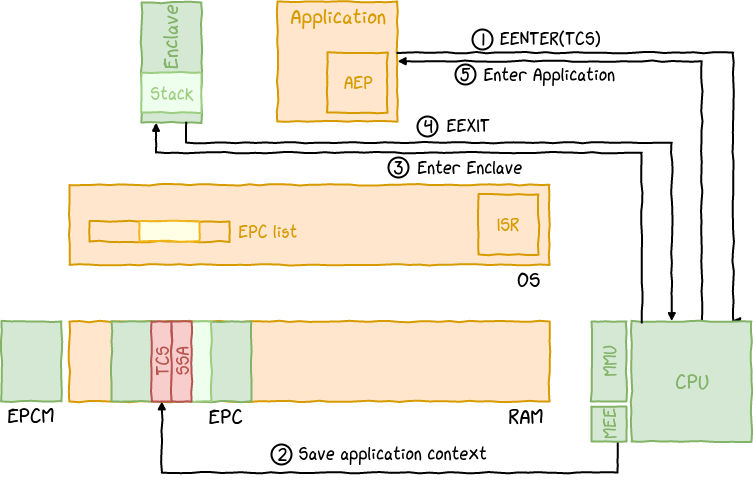
\includegraphics[scale=0.35]{Images/procedure.png}
            \end{center}
        \end{column}
        \end{columns}
\end{frame}

\begin{frame}
    \frametitle{Local Attestation}
    \begin{itemize}
        \visible<1->{\item Enclaves can communicate to each other}
        \visible<2->{\item Local attestation is a proof, that the other enclave exists and is trustable}
        \visible<3>{\item A channel must have been established between the two enclaves}
    \end{itemize}
\end{frame}

\begin{frame}
    \frametitle{Local Attestation}
    \begin{enumerate}
        \visible<1->{\item The first enclave can ask the hardware to generate a credential, named report, and send it to the other enclave}
        \visible<2->{\item The second can verify, that this resport is generated on the same platform and can now trust this enclave}
        \visible<3>{\item The second enclave has also to proof the report of the first enclave}
    \end{enumerate}
\end{frame}

%vielleicht mit Bild als erklärung leichter????????

\begin{frame}
    \frametitle{Remote Attestation}
    \begin{itemize}
        \visible<1->{\item Remote attestation is an exchange of a ``quote``}
        \visible<2->{\item Remote attestation needs an extra architectural enclave, called ``quoting enclave``}
        \visible<3->{\item This extra enclave is an architectural enclave, called ``quoting enclave``}
        \visible<4->{\item The quoting enclave verifies and transforms the enclave report into a quote}
        \visible<5->{\item A quote is signed by the quoting enclave by the Provisioning Key}
        \visible<6>{\item This quote is remotely verifiable}
    \end{itemize}
\end{frame}

\begin{frame}
    \frametitle{Remote Attestation}
    \begin{enumerate}
        \visible<1->{\item An attestation request is send from a server to the application}
        \visible<2->{\item The application sends a report request to the application enclave}
        \visible<3->{\item The application enclave returns the generated report}
        \visible<4->{\item The application receives the report and forwards it to the quoting enclave to be signed}
        \visible<5->{\item The quoting enclave generates from the report a quote and the quote is send back to the application}
        \visible<6->{\item The application sends the quote to the server for verification}
        \visible<7->{\item The server validates the quote signature and the server sends the data to the attestation service}
    \end{enumerate}
\end{frame}

%vielleicht mit Bild als erklärung leichter????????

\begin{frame}
    \frametitle{Sealing}
    \begin{itemize}
        \visible<1->{\item Process of encrypting enclave secrets for persistent sorage is calles sealing}
        \visible<2->{\item Different ways of sealing}
        \visible<3->{\item Enclave retrieves the seal Key using the EGETKEY instruction, which returns a cryptographical key}
        \visible<4>{\item Key is used to encrypt and ensure data integrity}
    \end{itemize}
\end{frame}

\begin{frame}
    \frametitle{Sealing - Different ways}
    \begin{itemize}
        \visible<1->{\item Enclave Identity}
        \visible<2->{\begin{itemize}
            \item Two distinct enclaves have different keys
            \item Sealed data will not be available to different versions of the same enclave
            \item Sealed data will only be available to identical enclave instantiations
        \end{itemize}}
        \visible<3->{\item Signer Identity}
        \visible<4->{\begin{itemize}
            \item Two distinct enclaves have different keys
            \item Two versions of an enclave share the same key
            \item multiple enclaves which are using the same key can all read each others data
        \end{itemize}}
        \visible<5->{\item Security Version Number (SVN)}
        \visible<6>{\begin{itemize}
            \item SVN is a counter which is incremented after each update
            \item Older versions of an enclave are not available to read data from a newer version
            \item keys are derived that an enclave can retrieve the keys corresponding to current or older security level
        \end{itemize}}
    \end{itemize}

    

\end{frame}

